\chapter{\acrshort{tpm} Software Stack}\label{ch:tss}

Il \acrshort{tcg} definisce un'interfaccia software per il \acrshort{tpm}v1.2, chiamata \acrlong{tss} (\acrshort{tss}), con lo scopo di fornire un'interfaccia verso il \acrshort{tpm} che permetta a quanti più programmatori un facile e immediato utilizzo, ma anche un'interfaccia che ponesse una base comune per tutte le piattaforme e per tutti i \acrshort{tpm}. Il \acrshort{tss} è quindi un'\acrshort{api} standard per accedere alle funzioni del \acrshort{tpm}, pensato per incentivare la diffusione di applicazioni adatte ad un \textit{computing} più resistente alla manomissione. Il \acrshort{tss} mira anche a fornire mezzi affinché le applicazioni possano comunicare con i \acrshort{tpm}, sia localmente che da remoto - una sfida non banale, se si pensa alla natura non sicura delle reti Internet.

Il \acrshort{tcg} lavora con l'obiettivo di produrre una specifica neutrale rispetto ai produttori hardware in modo che i venditori di applicazioni possano scrivere applicazioni che funzioneranno indipendentemente dalla piattaforma, dal sistema operativo o dall'ambiente utilizzato. 

Operativamente il \acrshort{tss} agisce da libreria, offrendo un'interfaccia di programmazione semplificata rispetto a quelli che altrimenti sarebbero dei comandi molto complicati e strutturati. Il \acrshort{tss} converte le chiamate ad alto livello applicativo in comandi equivalenti per il \acrshort{tpm}, li invia al driver del dispositivo, che poi li trasmette fisicamente al chip.

I livelli della libreria sono: Feature \acrshort{api} (FAPI), Enhanced System API (ESAPI), System API (SAPI), \acrshort{tpm} Command Transmission Interface (TCTI), \acrshort{tpm} Access Broker (TAB), Resource Manager (RM) e Device Driver (DD).

Il Device Driver potrebbe avere un nome fuorviante: non è da intendere come i driver utilizzati dai \acrshort{so} per interfacciarsi con l'hardware. Anzi, questo è il componente che gestisce la trasmissione fisica dei dati.

\begin{figure}[htbp]
    \centering
        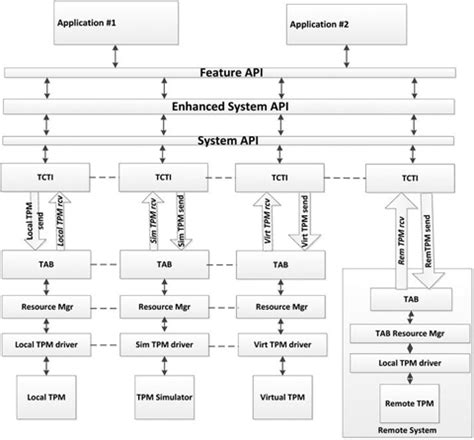
\includegraphics[width=0.7\textwidth]{figures/diagramma-tss.png}
    \caption{Diagramma del \acrshort{tss}, con un esempio per \acrshort{tpm} locale, un simulatore, un \acrshort{tpm} virtuale ed uno remoto.}
    \label{fig:diagramma_tss}
\end{figure}

\section{FAPI -- Feature API}\label{sec:fapi}

Il livello Feature \acrshort{api} (\acrshort{fapi}) nello stack software \acrshort{tpm} fornisce un set di \acrshort{api} di alto livello progettate per semplificare l'interazione con le funzionalità del \acrshort{tpm}. Questo livello offre un'interfaccia \textit{user-friendly} per sviluppatori, permettendo loro di accedere facilmente alle funzionalità di sicurezza avanzate del \acrshort{tpm} senza dover gestire la complessità delle \acrshort{api} di basso livello.

Su questo livello si scrivono la maggior parte delle applicazioni utente: è pensato proprio per essere il punto in cui i programmatori accedono alle funzionalità più comunemente utilizzate del \acrshort{tpm}. E' costruito pensando che la maggior parte dei programmi che usano il \acrshort{tpm}, non abbiano bisogno delle \acrshort{api} più profonde.

Il \acrshort{fapi} cerca anche di minimizzare il numero di chiamate che un'applicazione deve fare per ottenere qualcosa, ed il numero di parametri che deve definire. Per questo un'implementazione potrebbe prevedere file di impostazione, che definiscono selezioni \textit{default} di algoritmi, dimensioni delle chiavi, modalità ecc. Un meccanismo comodo per gli utenti finali che non dovrebbero più preoccuparsi di definire i dettagli di utilizzo del \acrshort{tpm} ad ogni chiamata.

Tutti gli oggetti creati e utilizzati dai comandi a livello \acrshort{fapi} devono essere autorizzati da una \textit{policy}, identificata dalla tag \texttt{TSS2\_POLICY\_AUTHVALUE}. I comandi per le \textit{policy} possono richiedere input esterno o no. Per il successo di questi comandi è necessario che il chiamante fornisca i parametri necessari -- tra i parametri ci sono proprio i valori su cui calcolare la correttezza della \textit{policy} -- perché il \acrshort{fapi} non è in grado di recuperare informazioni esterne.

Qui entra in gioco un meccanismo di \textit{callbacks}: le \textit{callback} sono registrate nel programma che parla con il \acrshort{fapi} cosicché questo possa sapere se serve una password, una selezione tra opzioni, o una firma. Ad esempio, per ottenere la password, la \textit{callback} è relativamente semplice, diventa sufficiente sfruttare una funzione - definita dall'applicazione che chiama l'\acrshort{api} -- per gestire l'interazione utente e recuperare l'input. 

Per quei comandi che non richiedono input esterno invece, le \textit{policy} fanno affidamento a dei \textit{check} sui valori nei \acrshort{pcr}, sulla \textit{locality} del comando, il \textit{counter} interno del \acrshort{tpm}, il codice che identifica il comando che richiede la verifica della \textit{policy}, l'hash del nome dell'oggetto inviato al \acrshort{tpm} ecc. Tutte queste modalità prevedono che sia il \acrshort{fapi} ad occuparsi della verifica richiesta.

Da notare che solitamente, una piattaforma possiede un solo \acrshort{tpm} che viene messo a disposizione di più applicazioni, con accesso mutualmente esclusivo. In realtà non è tassativo, e da una singola macchina si potrebbero usare \acrshort{tpm} simulati, remoti o fisici senza alcun limite.

\section{\acrshort{esapi} - Enhanced System \acrshort{api}}\label{sec:esapi}

Il livello Enhanced System \acrshort{api} (\acrshort{esapi}) fornisce \acrshort{api} di medio livello che offrono un maggiore controllo e funzionalità rispetto alle \acrshort{api} di basso livello (\acrshort{sapi}). 

Permette di gestire le sessioni in minima parte e supporta alcune delle capacità crittografiche rese disponibili dal \acrshort{tpm}. 

Questo livello è progettato e pensato per sviluppatori che necessitano di operazioni più dettagliate e personalizzate sulle funzionalità del \acrshort{tpm}, pur mantenendo un'interfaccia abbastanza semplice e senza necessitare di uno studio approfondito della specifica.

Il livello \acrshort{esapi} rappresenta le risorse che utilizza come una \textit{linked list}: ogni nodo consiste in una struttura contenente un \textit{handle} (un identificatore univoco per il nodo), la risorsa da memorizzare e un puntatore all'elemento successivo. 

\section{\acrshort{sapi} -- System \acrshort{api}}\label{sec:sapi}

Il livello System \acrshort{api} (\acrshort{sapi}) rappresenta un'\acrshort{api} di basso livello con accesso diretto e dettagliato alle funzioni del \acrshort{tpm}. È progettato per sviluppatori che necessitano del massimo controllo sulle operazioni del \acrshort{tpm}, permettendo loro di interagire direttamente con le primitive di sicurezza e gestire le risorse del \acrshort{tpm}. Viene richiamata ed utilizzata ogni volta che sono effettuate chiamate a basso livello come firmware, BIOS, applicazioni, sistemi operativi, ecc. 

Il \acrshort{sapi} è concettualmente ma anche concretamente uno spartiacque: i livelli sopra il \acrshort{sapi} esistono generalmente con corrispondenza uno ad uno per ogni processo che fa utilizzo del \acrshort{tpm}. I livelli al di sotto, sono solitamente specifici per piattaforma che dispone di \acrshort{tpm}.

La specifica del \acrshort{sapi} è pensata per essere utilizzabile su diverse piattaforme. Da sottolineare lo sforzo progettuale per permettere di minimizzare l'utilizzo della memoria: le implementazioni del \acrshort{sapi} possono evitare di allocare memoria, delegando la responsabilità al programma chiamante.

I comandi disponibili nel \acrshort{sapi} si dividono in quattro gruppi: \textit{context allocation functions}, \textit{preparation functions}, \textit{execution functions} e \textit{completion functions}. Di seguito una breve panoramica:

\begin{description}
    \item[\textit{context allocation functions}:] comandi che si occupano di allocare la struttura dati di \textit{context} necessaria per un comando \acrshort{sapi}. La struttura è definita dalle singole implementazioni e indica come vengono memorizzati i dati dello stato \acrshort{tpm} necessari per la corretta esecuzione di un comando.
    
    \item[\textit{preparation functions}:] alcune funzionalità del \acrshort{tpm} possono necessitare dello svolgimento di \textit{pre-processing} e \textit{post-processing}. Il meccanismo di ``preparazione'' dei parametri di un comando è chiamato \textit{marshalling}, e le \textit{preparation functions} hanno proprio questo ruolo: predispongono i parametri, ordinano flussi di byte, strutturano i dati, preparano le sessioni. Sono fondamentali per iniziare e concludere alcune chiamate di comandi \acrshort{tpm}.
    
    \item[\textit{execution functions}:] sono quei comandi che effettuano l'invio del comando e ne riceve le risposte - l'invio può essere sincrono o asincrono. Ci sono due modi per inviare comandi in modo sincrono: la prima prevede una sequenza di chiamate di funzione domanda-risposta (\textit{multi-chiamata}); la seconda è una chiamata unica. La necessità di supportare la modalità asincrona rispetto a quella sincrona e per la chiamata unica rispetto a un approccio \textit{multi-chiamata} non nasce da un motivo di progettazione, ma dall'idea di implementare il \acrshort{tss} per il maggior numero possibile di architetture applicative.
    
    \item[\textit{completion functions}:] gruppo di funzioni atte ad abilitare il \textit{post-processing} di un altro comando qualora necessario: ad esempio quando viene richiesto un calcolo \acrshort{hmac}, o una decifratura con verifica di integrità. Queste funzioni usano i parametri puntatore e dimensione del parametro di risposta, per prelevare i dati che vanno post-processati ed eseguire verifiche, calcoli o controlli che richiesti.
\end{description}

\section{\acrshort{tcti} -- \acrshort{tpm} Command Transmission Interface}\label{sec:tcti}

L'interfaccia \acrshort{tpm} Command Transmission Interface (\acrshort{tcti}) rappresenta un componente fondamentale del \acrshort{tss}, di fatto perché gestisce la trasmissione e la ricezione dei comandi tra l'applicazione.

La \acrshort{tcti} funge da ponte per l'invio di flussi di byte (un comando \acrshort{tpm} è un flusso di byte) dal \acrshort{tpm} alle applicazioni e viceversa. Fornisce un'interfaccia standardizzata che consente alle applicazioni di interagire con il \acrshort{tpm} senza che queste debbano gestire i dettagli specifici della comunicazione con il dispositivo, semplificando anche l'uso dei comandi. Lavora a basso livello ed è l'\acrshort{api} usata dal \acrshort{sapi} per comunicare con il \acrshort{tpm} (per usare \acrshort{tcti} serve conoscere cose sulle interfacce driver).

La \acrshort{tcti} stessa non fornisce meccanismi di autenticazione o cifratura. Tuttavia, le applicazioni che utilizzano la \acrshort{tcti} possono implementare la loro autenticazione e cifratura sui dati trasmessi.

Questa interfaccia a basso livello è utilizzata dal \acrshort{sapi} per la comunicazione con il \acrshort{tpm}. Quando un'applicazione invoca una funzione \acrshort{sapi}, deve fornire un \acrshort{tcti} \textit{context} che include puntatori a funzioni cruciali come \texttt{transmit} e \texttt{receive}. Questi puntatori permettono alla \acrshort{sapi} di inviare comandi al \acrshort{tpm} e di ricevere le risposte. Se l'applicazione deve comunicare con più \acrshort{tpm}, può creare \acrshort{tcti} \textit{contexts} distinti, ciascuno configurato con i puntatori di funzione appropriati per il tipo di \acrshort{tpm} di riferimento.

La struttura del \acrshort{tcti} \textit{context} comunque è associata ad un processo ed un solo \acrshort{tpm} alla volta. Viene configurata in fase di inizializzazione e può essere definita sia al momento della compilazione del codice implementativo che dinamicamente durante l'avvio del sistema operativo. Questo processo di configurazione e la successiva scoperta del \acrshort{tpm}, locale o remoto, avviene prima dell'uso della \acrshort{sapi} e non è oggetto della specifica \acrshort{tcti} - dovrà essere qualche altro componente ad occuparsene. La struttura del contesto \acrshort{tcti} include tutti i puntatori a funzioni (oltre a quelle di \texttt{transmit} e \texttt{receive} già citate) che forniscono servizi per la gestione della trasmissione dei comandi \acrshort{tpm}.

Nota: essendo il \acrshort{tcti} indipendente dalla tecnologia \acrshort{tpm} che effettivamente viene utilizzata, è possibile un sistema necessiti di passare dall'utilizzo di un d\acrshort{tpm} ad un v\acrshort{tpm}. Il \acrshort{tcti} non cambia la sua funzione di base, ma il driver che gestisce la comunicazione con il \acrshort{tpm} cambierà.

In sintesi, il v\acrshort{tpm} richiede un sistema di virtualizzazione in grado di gestire l'accesso a più istanze di \acrshort{tpm} emulati, con il \acrshort{tcti} che deve essere configurato per supportare questa modalità. Tale configurazione dipende dal sistema di virtualizzazione utilizzato (come KVM o Xen) e dai driver di emulazione \acrshort{tpm}. Inoltre, il \acrshort{tcti} deve adattarsi a nuovi driver, interfacce di comunicazione e, eventualmente, a modalità di gestione delle risorse hardware o virtuali. La transizione a un v\acrshort{tpm} implica quindi una configurazione accurata del \acrshort{tcti}, affinché possa interagire correttamente con il \acrshort{tpm} virtuale, garantendo la compatibilità con il sistema in esecuzione e la gestione continua e senza interruzioni della comunicazione con il \acrshort{tpm}.

\section{\acrshort{tab} -- \acrshort{tpm} Access Broker}\label{sec:tab}

Il \acrshort{tpm} Access Broker è il componente progettato per gestire l'accesso concorrente al \acrshort{tpm} da parte di più processi. Il loro scopo principale è garantire che le applicazioni e i processi possano interagire con il \acrshort{tpm} senza doversi preoccupare della complessità derivante dalla gestione dell'accesso multiplo con mutua esclusione.

In molte implementazioni, il \acrshort{tab} e il Resource Manager (\acrshort{rm}) sono strettamente integrati in un unico modulo software. Solitamente questa architettura ha senso perché una tipica implementazione del \acrshort{tab} può consistere in alcune semplici modifiche al \acrshort{rm}.

A seconda della progettazione del sistema, \acrshort{tab}-\acrshort{rm} (o solo \acrshort{tab}) possono risiedere nello strato superiore di uno stack di driver del dispositivo \acrshort{tpm} o essere implementati come un processo \textit{daemon} che funge da intermediario tra lo strato \acrshort{api} del Trusted Software Stack (\acrshort{tss}) e il driver del dispositivo \acrshort{tpm} sottostante.

Come già definito, la funzione principale del \acrshort{tab} è arbitrare l'accesso al \acrshort{tpm} tra i vari processi. Durante l'invio di un comando e la ricezione di una risposta, il \acrshort{tab} garantisce che nessun altro processo possa interferire, assicurando così un accesso ordinato e sincronizzato al \acrshort{tpm}. Inoltre, il \acrshort{tab} impedisce ai processi di accedere a sessioni o oggetti \acrshort{tpm} che non possiedono. Il \acrshort{tab} verifica l'autorizzazione ad accedere controllando che la connessione \acrshort{tcti} utilizzata per caricare gli oggetti stessi o avviare le sessioni sia la stessa da cui proviene la richiesta.

È importante sottolineare che, come vale per \acrshort{tcti}, il modulo \acrshort{tab} (o equivalentemente il modulo combinato \acrshort{tab}-\acrshort{rm}) non fornisce meccanismi di autenticazione o cifratura. Questa scelta è motivata da alcuni ragionamenti circa la funzione del \acrshort{tab} (ma vale anche per \acrshort{tcti}): 
il modulo deve essere trasparente e semplice per non complicare il \textit{design} o introdurre \textit{overhead} inutile; 
il \acrshort{tss} cerca di separare al massimo le responsabilità dei suoi livelli, il \acrshort{tab} si occupa dell'arbitraggio delle risorse. In generale sono le applicazioni o i componenti di sicurezza del \acrshort{so} ad occuparsi di queste funzionalità;
l'assenza di meccanismi di sicurezza intrinseci sicuramente rende più semplice implementare soluzioni personalizzate per ogni applicazione e adattarsi meglio al contesto in cui si sviluppa;

Tuttavia l'assenza di una cifratura a livello fisico dei dati, rende l'architettura del \acrshort{tpm} tradizionale per Personal Computers particolarmente debole agli attacchi \textit{bus sniff}. Ne verrà analizzato un esempio più avanti. Risulta comunque essere un attacco che nella maggior parte dei casi, richiede molta preparazione da parte dell'attaccante ed una buona finestra di tempo di accesso incontrollato al dispositivo. Sicuramente se si analizzano contesti di \acrshort{tpm} virtualizzati o remoti, l'analisi del rischio cambia, e l'impatto risulta diverso.

\section{\acrshort{rm} - Resource Manager}\label{sec:rm}

Il Resource Manager (\acrshort{rm}) svolge un ruolo cruciale nella gestione della memoria del \acrshort{tpm}. Poiché i \acrshort{tpm} dispongono di risorse ridotte, il \acrshort{rm} deve gestire con molta cura la memoria interna del chip scambiando dinamicamente oggetti e sessioni tra il \acrshort{tpm} e la memoria di sistema, in modo simile a un gestore della memoria virtuale in un sistema operativo. Il \acrshort{rm} può non essere necessario se il \acrshort{tpm} si trova in una scheda dove l'accesso sarà effettuato sempre e solo da un 

Un \acrshort{tpm} può gestire al massimo tre \textit{handle} di entità e tre \textit{handle} di sessione contemporaneamente. Per eseguire un comando, tutte queste risorse devono essere presenti nella memoria interna del \acrshort{tpm}. Il compito del \acrshort{rm} è intercettare il flusso di byte, identifica quali risorse devono essere caricate nel \acrshort{tpm}, scambiare gli elementi meno prioritari per liberare spazio e caricare gli oggetti richiesti. Nel caso di oggetti e sequenze, poiché il loro \textit{handle} può cambiare dopo essere stati ricaricati, l'\acrshort{rm} deve anche virtualizzare gli \textit{handle} prima di restituirli al chiamante, garantendo una mappatura corretta delle risorse.

Come già menzionato, il \acrshort{rm} è spesso integrato con il \acrshort{tab} in un unico modulo software. Di solito, esiste un \acrshort{tab}-\acrshort{rm} per ogni \acrshort{tpm}, ma in alcuni casi un singolo \acrshort{tab}-\acrshort{rm} può gestire più \acrshort{tpm}. In questo scenario, il modulo deve tenere traccia degli \textit{handle} associati a ciascun \acrshort{tpm}, garantendo una separazione chiara tra le risorse, anche se il metodo specifico per farlo non rientra nelle specifiche \acrshort{tss}.

Il \acrshort{tab} e il \acrshort{rm} lavorano in modo trasparente per gli strati superiori dello stack software. Senza un \acrshort{tab}-\acrshort{rm}, la sincronizzazione tra processi e l'arbitraggio dell'accesso al \acrshort{tpm} dovrebbero essere gestiti manualmente dall'applicazione, aumentando la complessità dello sviluppo.

L'uso del \acrshort{tab}-\acrshort{rm} è particolarmente utile negli ambienti \textit{multithread} o \textit{multiprocess}, poiché semplifica la gestione delle risorse e isola gli sviluppatori dai dettagli di basso livello. Tuttavia, nelle applicazioni \textit{mono-thread} e integrate, dove il \acrshort{tpm} è utilizzato da un solo processo, l'implementazione di un \acrshort{tab}-\acrshort{rm} può essere evitata per ridurre il sovraccarico computazionale.

\section{\acrshort{dd} - Device Driver}\label{sec:dd}

Nel processo di comunicazione con il \acrshort{tpm}, il livello più basso dello stack software è rappresentato dal Device Driver (\acrshort{dd}), che gestisce la trasmissione fisica dei dati da e verso il chip \acrshort{tpm}. Dopo che i livelli superiori hanno svolto il loro lavoro, l'ultimo collegamento entra in gioco: il \acrshort{dd} riceve un \textit{buffer} di byte di comando e una lunghezza del \textit{buffer} ed esegue le operazioni necessarie per inviare quei byte al \acrshort{tpm}. Quando richiesto dai livelli superiori nello stack, il \acrshort{dd} rimane in attesa fino a quando il \acrshort{tpm} è pronto, legge i byte della risposta e li restituisce al livello superiore dello stack.

Le interfacce fisiche e logiche che il \acrshort{dd} utilizza per comunicare con il \acrshort{tpm} sono al di fuori dell'ambito delle specifiche della libreria \acrshort{tpm} e sono definite nelle specifiche della piattaforma che implementa \acrshort{tpm}. Attualmente, per i \acrshort{tpm} utilizzati nei PC, le due principali opzioni di interfaccia sono FIFO8 e Command Response Buffer (\acrshort{crb}). 

L'interfaccia FIFO8 utilizza un meccanismo \textit{first-in, first-out} per trasmettere i dati, con un indirizzo fisso \textit{hardcoded} per invio e ricezione e altri indirizzi per operazioni di \textit{handshake} e monitoraggio dello stato del \acrshort{tpm}. È rimasta pressoché invariata fino al \acrshort{tpm} 2.0 e può operare su bus come SPI o LPC.

L'interfaccia \acrshort{crb}, introdotta con il \acrshort{tpm} 2.0, usa invece \textit{buffer} di memoria condivisa per comunicare i comandi e le risposte, offrendo maggiore efficienza e una gestione più strutturata rispetto alla FIFO.

\section{Un'implementazione TSS}\label{sec:imp_tss}

L'implementazione \texttt{tpm2-tools}, rappresenta una delle soluzioni principali per interagire con il \acrshort{tpm} 2.0, attraverso una serie di strumenti a riga di comando. \texttt{tpm2-tools} non è parte della specifica \acrshort{tss}, bensì è un'implementazione \textit{open source} sviluppata nell'ambito del più ampio ecosistema \texttt{tpm2-software}.

Consente di eseguire operazioni complesse sul \acrshort{tpm} senza dover scrivere codice a basso livello, semplificando così l'adozione di questa tecnologia in diversi contesti di sicurezza informatica.

La suite \texttt{tpm2-tools} si basa sull'architettura standard della \acrshort{tss} e il Resource Manager (\acrshort{rm}) gioca un ruolo essenziale, gestendo l'accesso concorrente al \acrshort{tpm} e virtualizzando le risorse per consentire un utilizzo efficiente in ambienti multiprocesso. In molti casi, questa funzione è svolta dal demone \texttt{tpm2-abrmd}, che si occupa di sincronizzare le richieste e di ottimizzare l'uso della memoria limitata del \acrshort{tpm}.

Per comunicare con il \acrshort{tpm}, \texttt{tpm2-tools} utilizza l'implementazione di \acrshort{tcti} fornita dal \acrshort{tcg}. A seconda del contesto, è possibile scegliere tra diverse modalità di interazione: l'accesso diretto al \acrshort{tpm} tramite il dispositivo \texttt{/dev/tpm0}, l'uso di un simulatore \acrshort{tpm} per ambienti di test, oppure il passaggio attraverso il \acrshort{rm} per una gestione più strutturata delle risorse.

\begin{figure}[htbp]
    \centering
    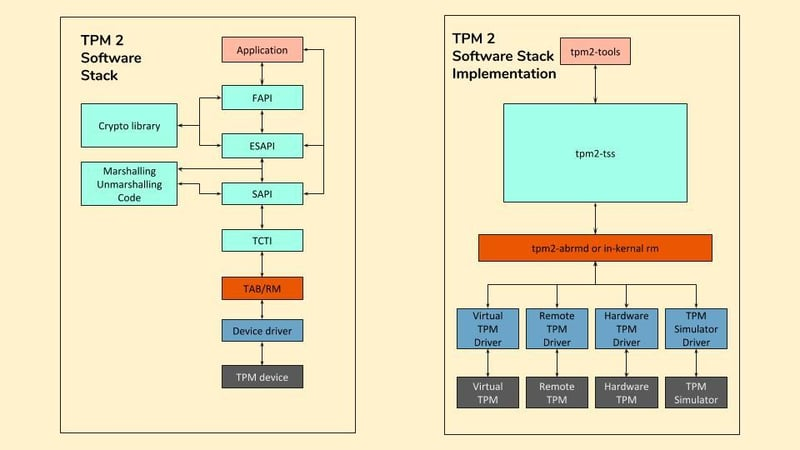
\includegraphics[width=0.77\textwidth]{figures/diagramma-tss-imp.png} % Inserisci qui il percorso della tua seconda immagine
    \caption{Diagramma \acrshort{tss} a sinistra e implementazione \texttt{tpm2-tools} a destra.}
    \label{fig:confronto_tss_tools}
\end{figure}

\texttt{tpm2-tools} è una suite potente ma presenta alcuni svantaggi che potrebbero limitarne l'uso in alcuni contesti. In primo luogo, essendo una suite a linea di comando, può risultare complessa per gli utenti che non sono familiari con i \textit{terminali} o con il funzionamento interno del \acrshort{tpm}.

Un altro aspetto limitante è che \texttt{tpm2-tools} opera principalmente a basso livello, il che significa che, per integrare il \acrshort{tpm} in applicazioni più complesse, potrebbe essere necessario scrivere codice aggiuntivo o fare affidamento su altre librerie. Questo lo rende meno adatto per chi cerca un'astrazione più alta e una soluzione pronta all'uso.

In termini di compatibilità, \texttt{tpm2-tools} è principalmente progettato per sistemi Linux, e potrebbe non essere ottimizzato o compatibile con altre piattaforme o dispositivi \acrshort{tpm}, limitandone l'utilizzo in ambienti eterogenei.

Un altro aspetto importante da considerare è che l'utilizzo di più strati di comunicazione nella suite può introdurre un certo \textit{overhead} di prestazioni, il che potrebbe essere problematico in ambienti dove è richiesta una gestione altamente performante delle risorse.

Infine, per sfruttare appieno le funzionalità di \texttt{tpm2-tools}, sono necessari strumenti esterni come il già citato \texttt{tpm2-abrmd}, che aggiungono un ulteriore livello di complessità alla configurazione e alla gestione del sistema.